\documentclass[times,twocolumn,final,authoryear]{elsarticle}

\usepackage{prletters}
\usepackage{framed,multirow}
%\usepackage{graphicx}
\usepackage[utf8]{inputenc}
\usepackage{amsmath}
%\usepackage[table]{xcolor}
%\usepackage{tabularx}
%\usepackage[backend=bibtex,style=model2-names]{biblatex}
\usepackage{subcaption}
\usepackage[colorinlistoftodos,prependcaption,textsize=tiny]{todonotes}
\usepackage{multirow}
\usepackage{makecell}
% \newcommandx{\unsure}[2][1=]{\todo[linecolor=red,backgroundcolor=red!25,bordercolor=red,#1]{#2}}
% \newcommandx{\change}[2][1=]{\todo[linecolor=blue,backgroundcolor=blue!25,bordercolor=blue,#1]{#2}}
% \newcommandx{\info}[2][1=]{\todo[linecolor=OliveGreen,backgroundcolor=OliveGreen!25,bordercolor=OliveGreen,#1]{#2}}
% \newcommandx{\improvement}[2][1=]{\todo[linecolor=Plum,backgroundcolor=Plum!25,bordercolor=Plum,#1]{#2}}
% \newcommandx{\thiswillnotshow}[2][1=]{\todo[disable,#1]{#2}}

% Formatting
% \setlength{\parindent}{4em}
%\setlength{\parskip}{1em}

%\newcommand{\X}{\cellcolor{blue!25}} 
%\newcolumntype{K}[1]{>{\centering\arraybackslash}p{#1}}
%\newcolumntype{C}{>{\centering\arraybackslash}X}

\linespread{0.98}
\hyphenation{ra-ting}

\captionsetup[figure]{labelfont=bf,textfont=bf,labelsep=period}
\captionsetup[table]{labelfont=bf,textfont=bf,justification=centering,labelsep=period,aboveskip=2pt}

\interfootnotelinepenalty=10000

\journal{Pattern Recognition Letters}

\begin{document}

\thispagestyle{empty}

\ifpreprint
  \setcounter{page}{1}
\else
  \setcounter{page}{1}
\fi

\begin{frontmatter}

\title{Continuous real-time annotation fusion correction via rank-based spatial warping}

\author[1]{Brandon M. \snm{Booth}\corref{cor1}} 
\cortext[cor1]{Corresponding author: 
  Tel.: +1-720-470-4284}
\ead{brandon.m.booth@gmail.com}
\author[1]{Karel \snm{Mundnich}}
\author[1]{Shrikanth S. \snm{Narayanan}}

\address[1]{Signal Analysis and Interpretation Lab, University of Southern California, 3740 McClinktock Avenue, EEB 400, Los Angeles, CA 90089, USA}

\received{1 May 2017}
\finalform{10 May 2017}
\accepted{13 May 2017}
\availableonline{15 May 2017}
\communicated{S. Sarkar}


\begin{abstract}
Human annotations are noisy and prone to influence from several factors including personal bias, task ambiguity, environmental distractions, health state, and more.  These annotations, however, are of integral value in human behavior studies, and in design and evaluation of machine learning applications, especially those involving hidden mental states that cannot effectively be measured or assessed by other means.  We propose a novel method for extending continuous real-time annotation fusion approaches to generate accurate ground truth estimates.  We validate our approach in a mechanically simple but perceptually demanding psychophysical annotation experiment where an objective truth is known.  Our method yields a ground truth in better agreement with the objective truth than state-of-the-art approaches and can be used to provide a more accurate fused annotation for real data.
\end{abstract}

\begin{keyword}
\MSC 41A05\sep 41A10\sep 65D05\sep 65D17
\KWD Annotation fusion\sep Behavior signal processing\sep Ordinal embedding
\end{keyword}

\end{frontmatter}

\section{Introduction}
Automated human behavior estimation and prediction problems for hidden state constructs such as emotional state, engagement, productivity, or attention are notoriously difficult and typically approached using supervised machine learning.  For these types of problems, self or expert annotations are often used to provide ratings for the target construct and establish a ground truth set of labels for machine learning.  However, the human annotation process is noisy and produces several types of label artifacts due to many factors such as perception bias, interpretation ambiguity, and distractions, to name a few.  The impact of these biases and cognitive effects on the annotations are magnified when the annotation task demands careful attention or vigilance over long sessions.  A time-economical annotation protocol is therefore paramount in order to obtain labels of the target construct that are consistent and congruent.  The usual strategy for combating these error sources involves gathering multiple annotations from different sources and fusing them to obtain a single ground truth.  Aggregation of multiple annotations helps mitigate the effect of noise and a careful fusion method ideally suppresses individual biases and artifacts, but there is yet no consensus on a best-practice fusion approach.

In this work, we focus on a continuous-scale annotation scheme where expert annotators observe recordings of an experiment session and annotate the target construct in real-time.  This annotation scheme has been used for mental constructs that evolve steadily over time like affective dimensions (arousal, valence, dominance) \citep{mckeown2012semaine, metallinou2013tracking, metallinou2013annotation, ringeval2013introducing, valstar2016avec}, and could be used for other mental states such as engagement, attention, productivity, or more generally whenever self-reports disrupt the natural flow of the target construct or introduce retroactive bias.  Continuous-scale real-time annotation affords extra freedom to the experts for subtle distinctions to be made while taking the full temporal context into account, but also is subject to further sources of noise and artifacts.

Prior work on continuous annotation has focused on ground truth estimation by modeling and removing general sources of lag, noise, and/or artifacts.  One approach from \cite{Mariooryad2015} finds an optimal time shift for separate annotations to align them before fusion via per-frame averaging.  This method corrects for variance in annotators' response times, but may perform poorly with adversarial annotations or changes in reaction lag over time (e.g. long annotation tasks).  Dynamic time warping \citep{DTW2007} is a well-known alignment solution that maximizes the agreement between annotators by handling variance in individual annotators' lag times, but also only corrects for temporal misalignments during fusion.  Long short-term memory networks (LSTMs) have also been proposed recently that correct for asynchronous annotator lag when fusing annotations using additional contextual information \citep{Ringeval2015}.  This approach seems to elegantly handle lag differences between annotators when fusing, but has only been shown to achieve good objective truth approximations when the contextual representation is appreciably informative of the underlying construct.

Furthermore, canonical correlation analysis (CCA) \citep{CCA1936} and correlated spaces regression (CSR) \citep{nicolaou2013correlated} focus on correcting systemic and consistent personal annotation biases by learning a projection function for a set of features that maximizes the projected features' correlation with the set of annotations.  These two approaches correct for spatial annotation biases and require a separate set of features to be extracted from the stimulus that are in some combination representative of the changes in annotation signal values.  Extensions of this tenet such as canonical time warping (CTW) \citep{CTW2009}, deep canonical correlation analysis (DCCA) \citep{andrew2013deep}, dynamic probabilistic canonical correlation analysis and time warping (DPCCA/DPCTW) \citep{nicolaou2014dynamic}, deep canonical time warping (DCTW) \citep{trigeorgis2016deep}, and generalized canonical time warping (GCTW) \citep{Zhou2016} have also been studied and shown to perform well on various data sets.  With the right set of features these methods can produce desirable fusions but often in human behavior studies these ideal features are as elusive as the estimation problems for which they are used, especially when annotation artifacts do not correlate with directly observable features of the stimulus.

Other methods use a shared latent state to model the ideal annotation signal and separate distortion states to learn annotators' biases and artifacts \citep{audhkhasi2013globally, zhu2015fusing, Gupta2016}.  For analytical convenience and to reduce sample complexity, these Bayesian network models assume exponential family priors for spatial distortion modeling, which are not necessarily reflective of the types of errors expert annotators make.  As volunteer-based crowd sourcing platforms such as Amazon's Mechanical Turk become more popular choices for large-scale annotation tasks, it becomes more difficult to model and fit a family of distortions to each annotator with confidence.

The fundamental problem confounding annotation fusion methods to date is the reliance on the average quality of continuous annotations.  Several studies have shown that people are better at comparative ranking than absolute rating \citep{Yannakakis2011, metallinou2013annotation, yannakakis2015ratings} suggesting that absolute continuous annotations may not exhibit coherence and self-consistency.  In this paper we affirm this idea by presenting the results from simple continuous annotation experiments showing high levels of agreement between annotators and a lack of consistency in labeling over time.  We then present a post-annotation correction method where additional relative rank information about interval subsets of the fused annotations are used to warp the result to better approximate the objective truths.  Rather than focusing on evaluating performance in latent state experiments, we validate our approach on experiments that are reflective of the types of perceptual problems that occur in hidden state annotation tasks, but where objective truths are known \textit{a priori}.  We further the utility of our approach by testing the robustness of our technique to noisy and incomplete additional information. This method is complementary to other fusion procedures and can be used to obtain better ground truth approximations.

\section{Experiment}
We used a simple but perceptually challenging annotation task where the objective truth was known for our study.  Ten annotators were asked to separately rate the intensity of the color green in real-time and on a continuous scale in two videos.  The videos were less than five minutes in length, 864x480 resolution, and comprised entirely of solid color frames of green at varying green channel values in RGB color space.  In each video, the green value was designed to change at different speeds and times while avoiding discontinuous changes.  The intention was to make the annotation process mechanically easy with the simple interface provided and to help ensure the main annotation challenge laid in the translation of green intensity perception to annotation rating.

The annotation process occurred in real time where annotators adjusted an interface in tandem with perceived changes in the video.  A slider widget representing a float value between zero (corresponding to black) and one (corresponding to full green) was displayed and annotators were instructed to watch the video and use a mouse to move the slider according to how green the video appeared.  No further instructions or clarifications were given. The value of the slider was recorded for each video frame at 30Hz, and a picture of the interface is shown in Figure \ref{fig:annotation_ui}.

\begin{figure}
	\centering
	\begin{subfigure}{0.49\columnwidth}
	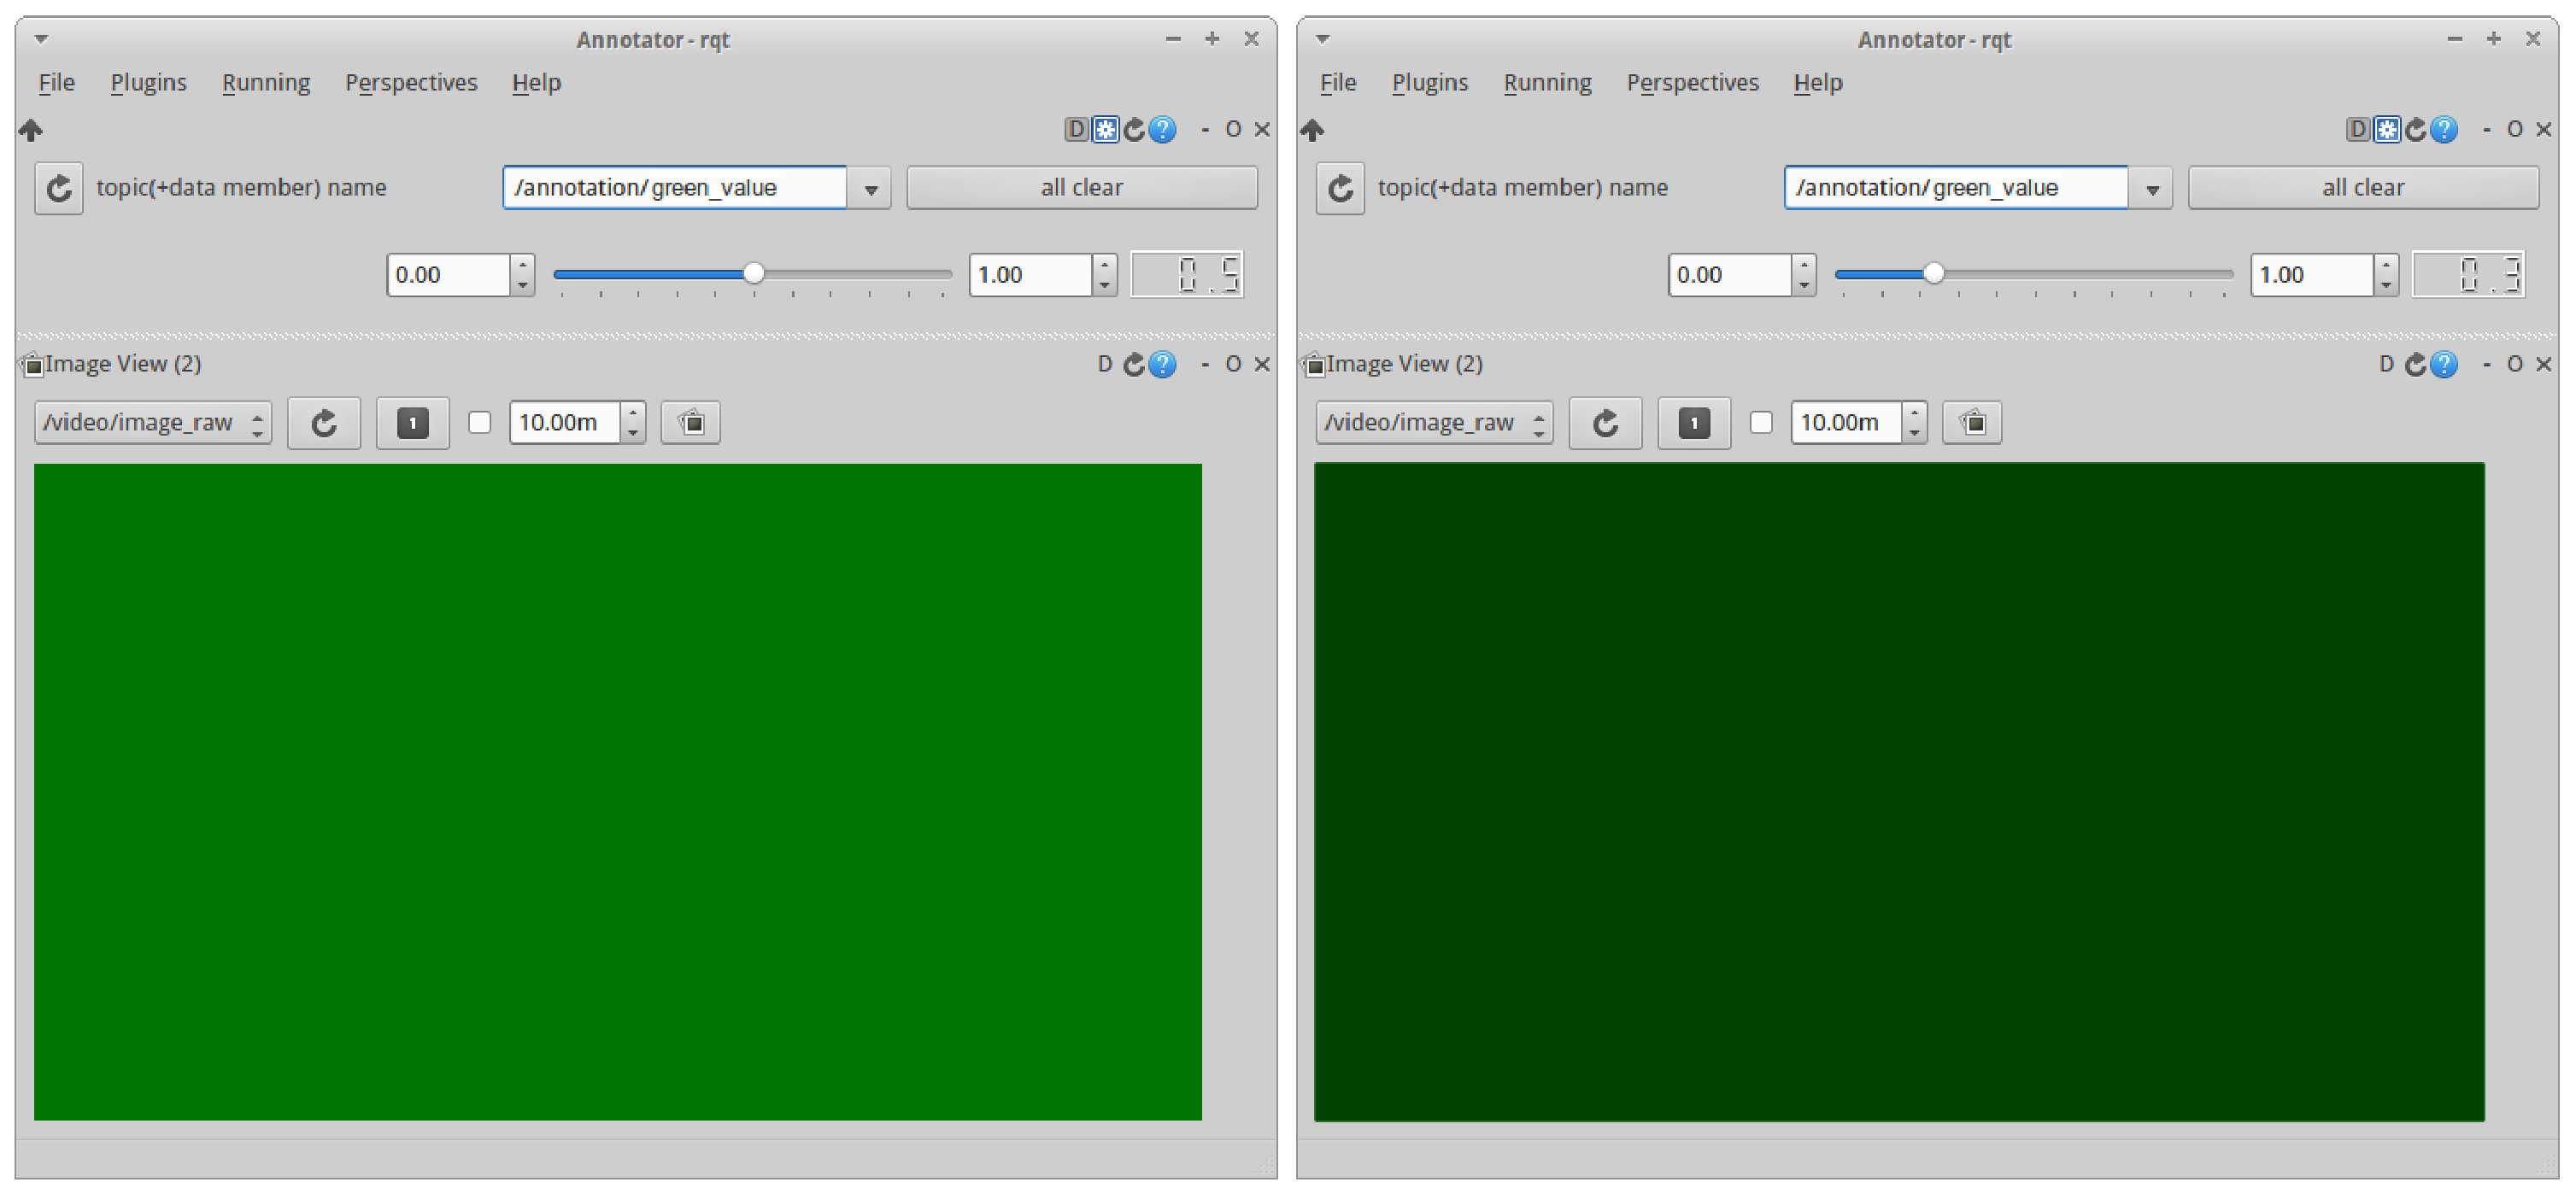
\includegraphics[width=\columnwidth]{images/green_ui}
	\end{subfigure}
	\begin{subfigure}{0.49\columnwidth}
	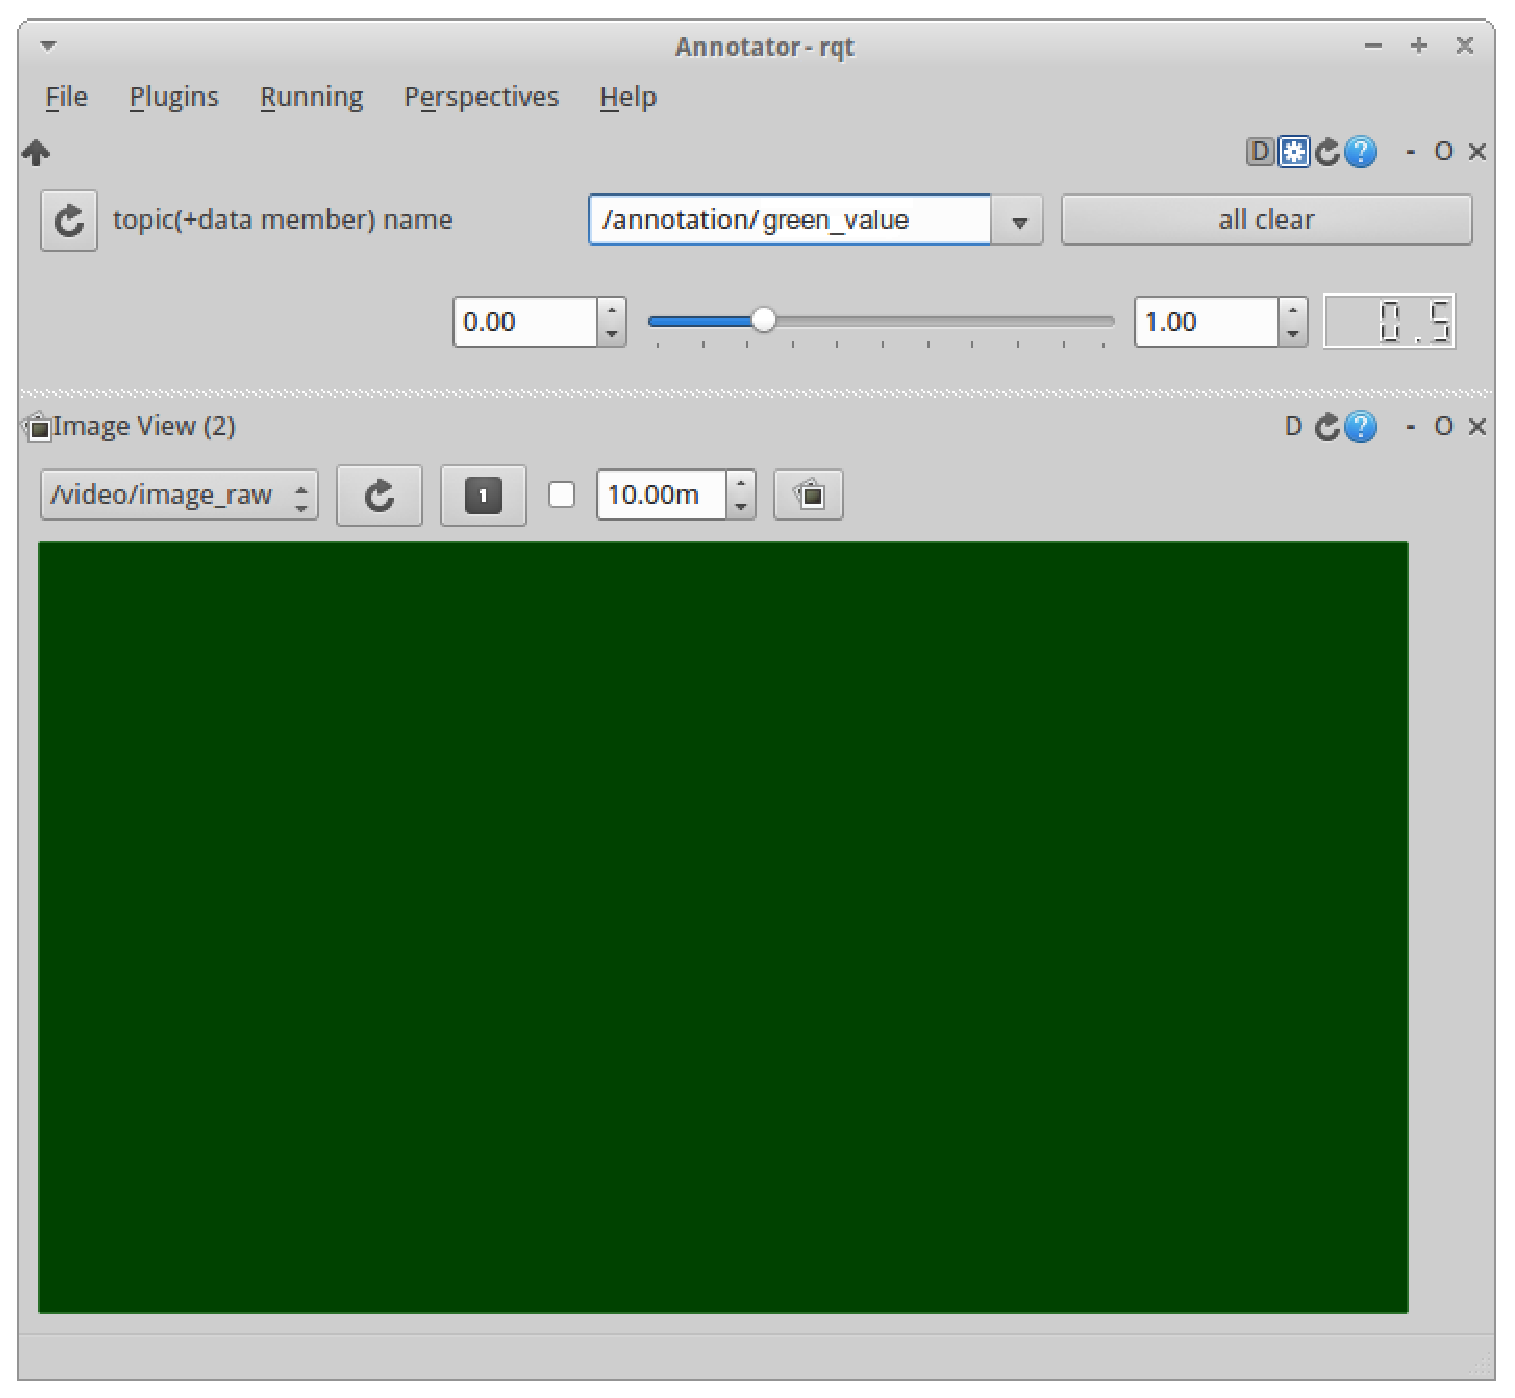
\includegraphics[width=\columnwidth]{images/green_ui2}
	\end{subfigure}
	\caption{Snapshot of the user interface at different times during the green channel value annotation task.  Annotators only adjusted the slider in sync with changes in the green video.}
	\label{fig:annotation_ui}
\end{figure}

Figure \ref{fig:annotations_ot} shows a plot of all ten annotations alongside the objective truth for both annotation tasks.  This plot suggests that annotators were generally quite good at capturing large changes and trends, but had difficulties in several areas.  First, most annotators tended to over-shoot the target value when annotating increases or decreases in value over a period of time thus suggesting they were fixated on annotating the rate of change rather than the actual rating.  Annotators were sensitive to and captured the appropriate direction of change, but sometimes were unable to estimate the correct rate of change.  Secondly, we note that approximately half of the annotators struggled to capture the lack of change in green value especially during the 100 to 150-second time interval in Figure \ref{fig:annotations_ot_a}.  One possible explanation is that the longer duration of this constant segment gave annotators time to realize their current rating did not match their perception and then adjust the value to match in spite of what was (not) occurring in the video.  Lastly, we note that similar green values were annotated inconsistently over time.  In particular, there was a significant difference in average annotation value per annotator between different time intervals where the green intensity was actually at a constant 0.5 value (see Figure \ref{fig:annotations_ot_a}).

\begin{figure*}[t]
	\centering
	\begin{subfigure}{0.49\textwidth}
	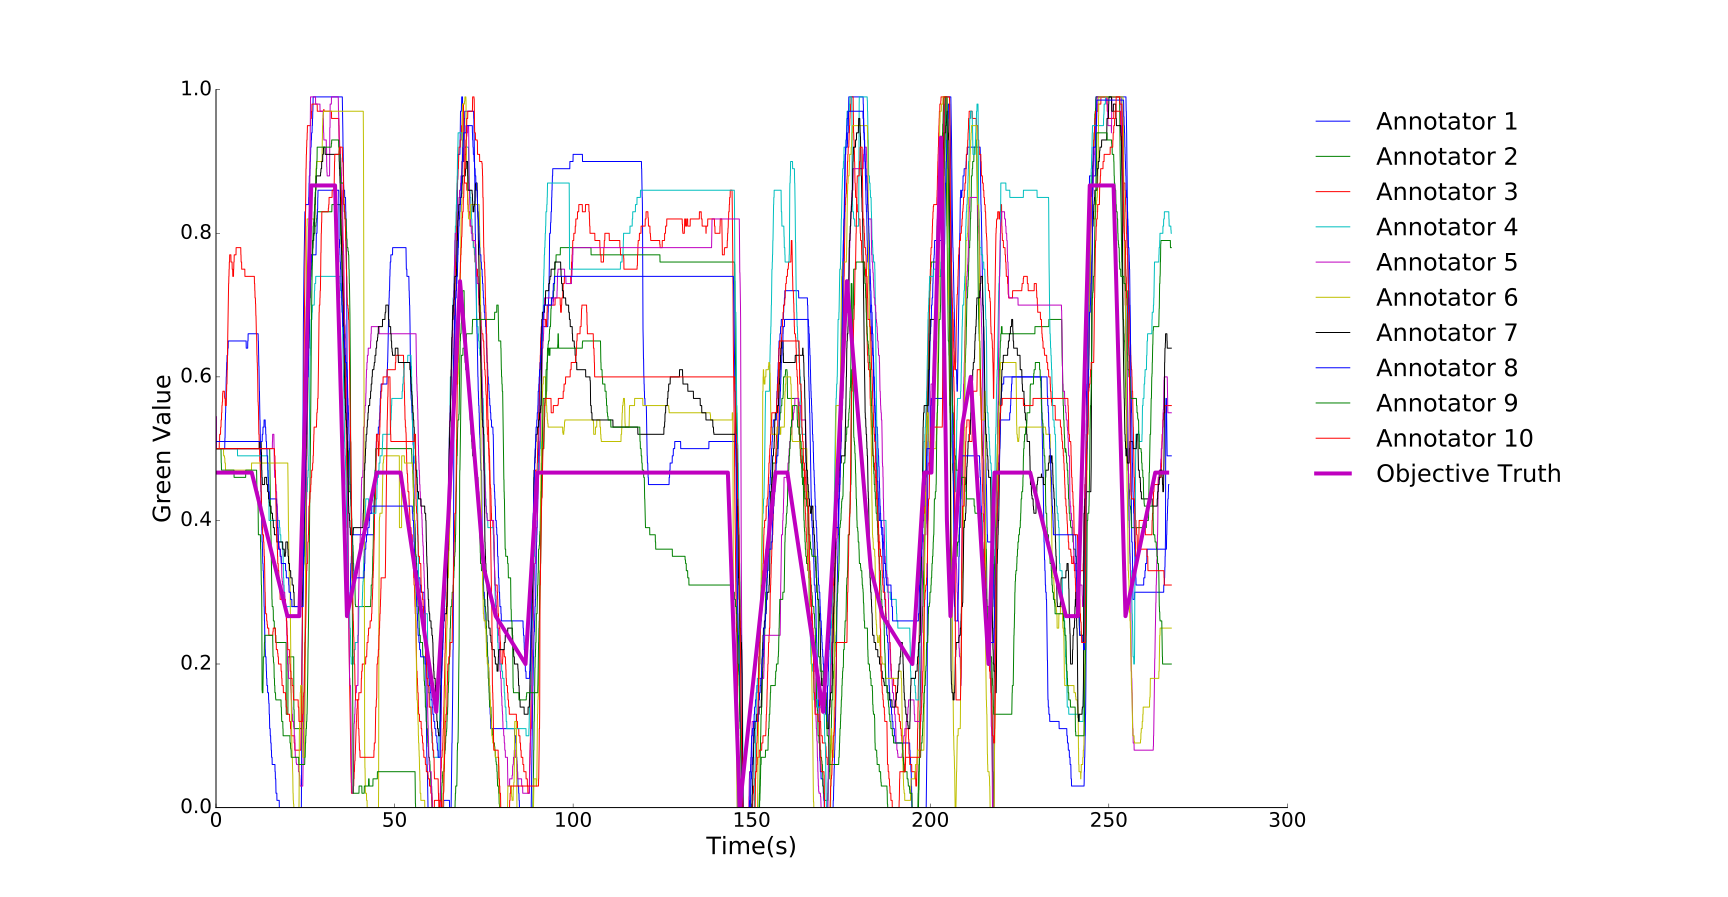
\includegraphics[width=\columnwidth]{images/annotations_ot}
	\caption{\footnotesize Task A \hspace*{1.2cm}}
	\label{fig:annotations_ot_a}
	\end{subfigure}
	\begin{subfigure}{0.49\textwidth}
	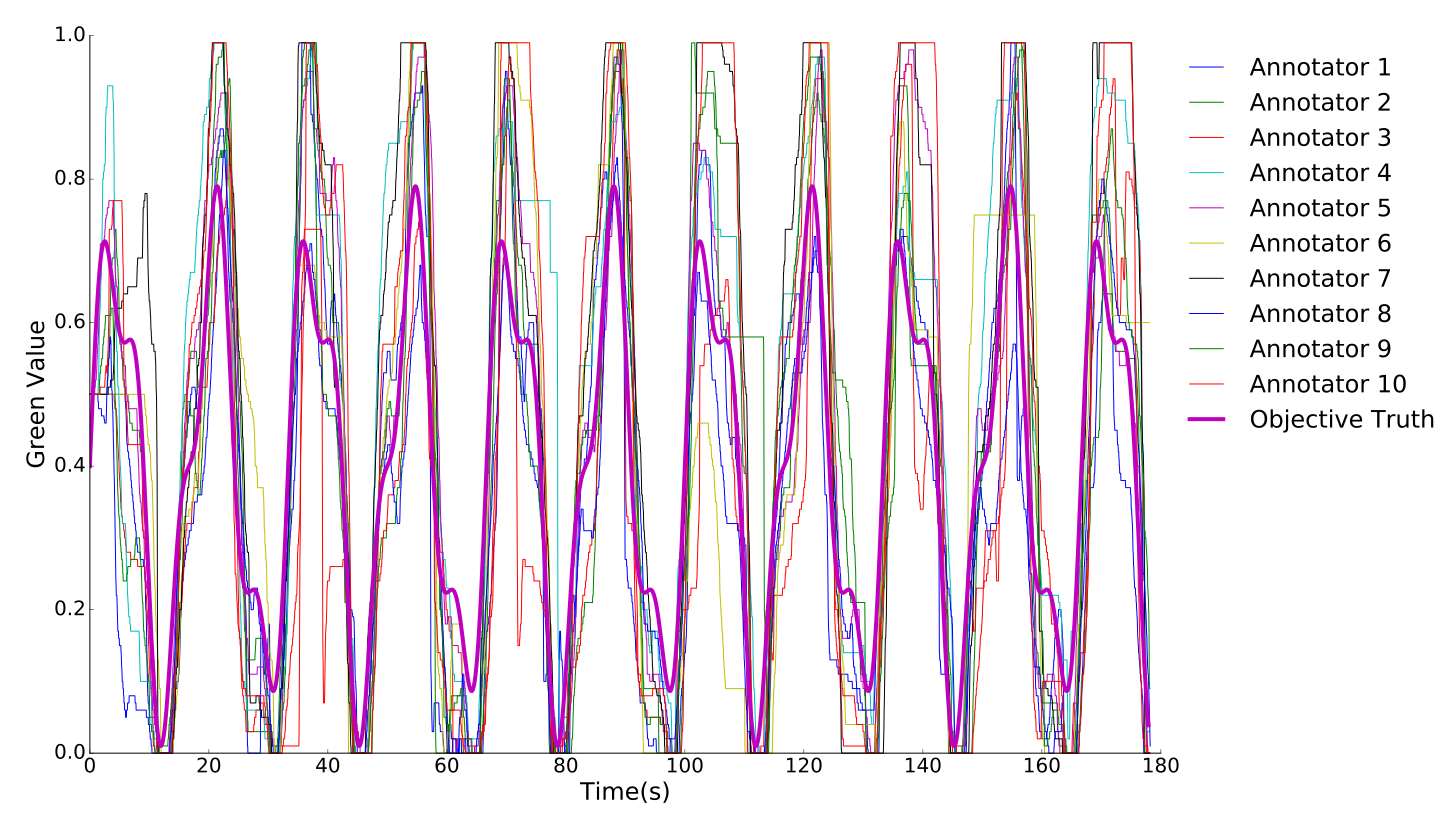
\includegraphics[width=\columnwidth]{images/annotations_ot2}
	\caption{\footnotesize Task B \hspace*{1cm}}
	\label{fig:annotations_ot_b}
	\end{subfigure}
	\caption{Annotations of green channel values alongside the true value in two separate annotation tasks.}
	\label{fig:annotations_ot}
\end{figure*}

This last observation implies that even for this relatively simple annotation task, it is difficult for annotators to accurately capture the trends while preserving self-consistency over time.  Given prior evidence that humans are better at ranking than rating \citep{Yannakakis2011, metallinou2013annotation, yannakakis2015ratings} and our own observations from this study, it is reasonable to assume that in continuous real-time annotation, experts are more focused and perhaps even better at faithfully capturing trends and less able to accurately assess the true value at any point in time.  We present a procedure for correcting these rating inconsistencies while preserving the more precise trend annotations.

\section{Fused Annotation Warping for Ground Truth Estimation}

We propose a method for warping fused annotations to establish a ground truth signal that has been corrected for various global inconsistencies, artifacts, and errors introduced during the real-time continuous human annotation process.  The method leverages a recurring observation that annotators more successfully capture trends and less accurately represent exact ratings \citep{Yannakakis2011, metallinou2013annotation, yannakakis2015ratings}.  In our approach, additional information must be collected from annotators after the continuous annotation task.  We leverage the structure of the fused annotations to identify segments of time in the video that can be treated as congruent units and thus reduce the amount of necessary additional information.  Further significant reductions to the required supplementary information are discussed in the results section.

Our method is summarized as a sequence of steps shown in Figure \ref{fig:pipeline}.
\begin{figure*}[t]
	\centering
	\includegraphics[width=\textwidth]{images/RankBasedSignalWarpingPipeline}
	\caption{Proposed pipeline for ground truth correction given continuous human annotations.}
	\label{fig:pipeline}
\end{figure*}
\iffalse
\begin{enumerate}
    \item Lag compensation and averaging
    \item Total variation (TV) denoising
    \item Constant interval extraction
    \item Triplet comparison collection
    \item Ordinal embedding
    \item Fused annotation warping
\end{enumerate}
\fi
The first step fuses the raw annotations together to form a single time series.  In this paper, this step simply time-aligns and averages all annotations to reduce systemic noise and limit the influence of random annotation artifacts.  Total variation (TV) denoising is then used to approximate the fused signal as a piecewise-constant step function.  Constant intervals are thereafter extracted from the denoised signal corresponding to time spans where annotators generally agree that the target construct does not noticeably change.  Additional rank information is then procured from annotators to re-evaluate the proper sorting of the these time intervals with respect to the target construct.  We collect comparison results among unique triplets of these constant intervals and employ an ordinal embedding technique to re-rank them.  Finally, the average signal is warped piecewise-linearly so the corresponding constant intervals align with the embedding.  These steps and their assumptions are described in detail in the corresponding sections below.

\subsection{Lag Compensation and Averaging (Annotation Fusion)}
The first step involves estimating an appropriate time shift for each annotation signal to align them with the video and compensate for lag due to human reaction times.  Several methods have been proposed for this \citep{DTW2007, CTW2009, andrew2013deep, nicolaou2014dynamic, Mariooryad2015, Ringeval2015, trigeorgis2016deep} and in principle any choice works for this step.  We use a simple per-annotator time shift (EvalDep) proposed by \cite{Mariooryad2015}.  This method requires some feature sequences to be extracted from the video for alignment, so we provide the green value and its forward difference per frame.  The average annotation lag is estimated at 1.6 seconds across annotators.  After shifting each annotation by its own lag estimate, we truncate the trailing frames so all annotations are equal length and then average them in time.  Note that the lag compensation is not strictly necessary but yields better final results. Figure \ref{fig:average_and_objective} shows the time-corrected average annotation signal for one of the annotation tasks.

\subsection{Total Variation Denoising}
Total variation denoising has been successfully used to remove salt and pepper noise from images while simultaneously preserving signal edges \citep{rudin1992nonlinear}.  In our context, we want to identify the set of nearly constant regions of the average annotation signal corresponding to a lack of noticeable change in the target construct.  TV denoising is preferable to other smoothing processes both because it approximates the function as a piecewise-constant step function as is desired, and also because it better preserves the structure of the signal.

We use the TFOCS MATLAB library \citep{becker2011templates} to find a new sequence $y_t$ that approximates a given sequence $x_t$ and minimizes:
\begin{equation*}
\min_{y_t} \Big[\sum_{t} ||x_t - y_t||_{\ell_2}^2 + \lambda\sum_{t} ||y_{t+1} - y_{t}||_{\ell_1}\Big]
\end{equation*}
The parameter $\lambda$ controls the influence of the temporal variation term and degree to which $y_t$ is approximately piecewise-constant.  In general this parameter needs to be tuned to produce a desirable sequence.  For this study, we hand-tune $\lambda$ and settle on a value of 0.05.  In principle, this parameter can be automatically selected based on other criteria and heuristics, but we leave this endeavor for future work.  Figure \ref{fig:tv_and_intervals} shows an example TV-denoised signal.

\begin{figure*}
	\centering
	\begin{subfigure}{0.49\textwidth}
	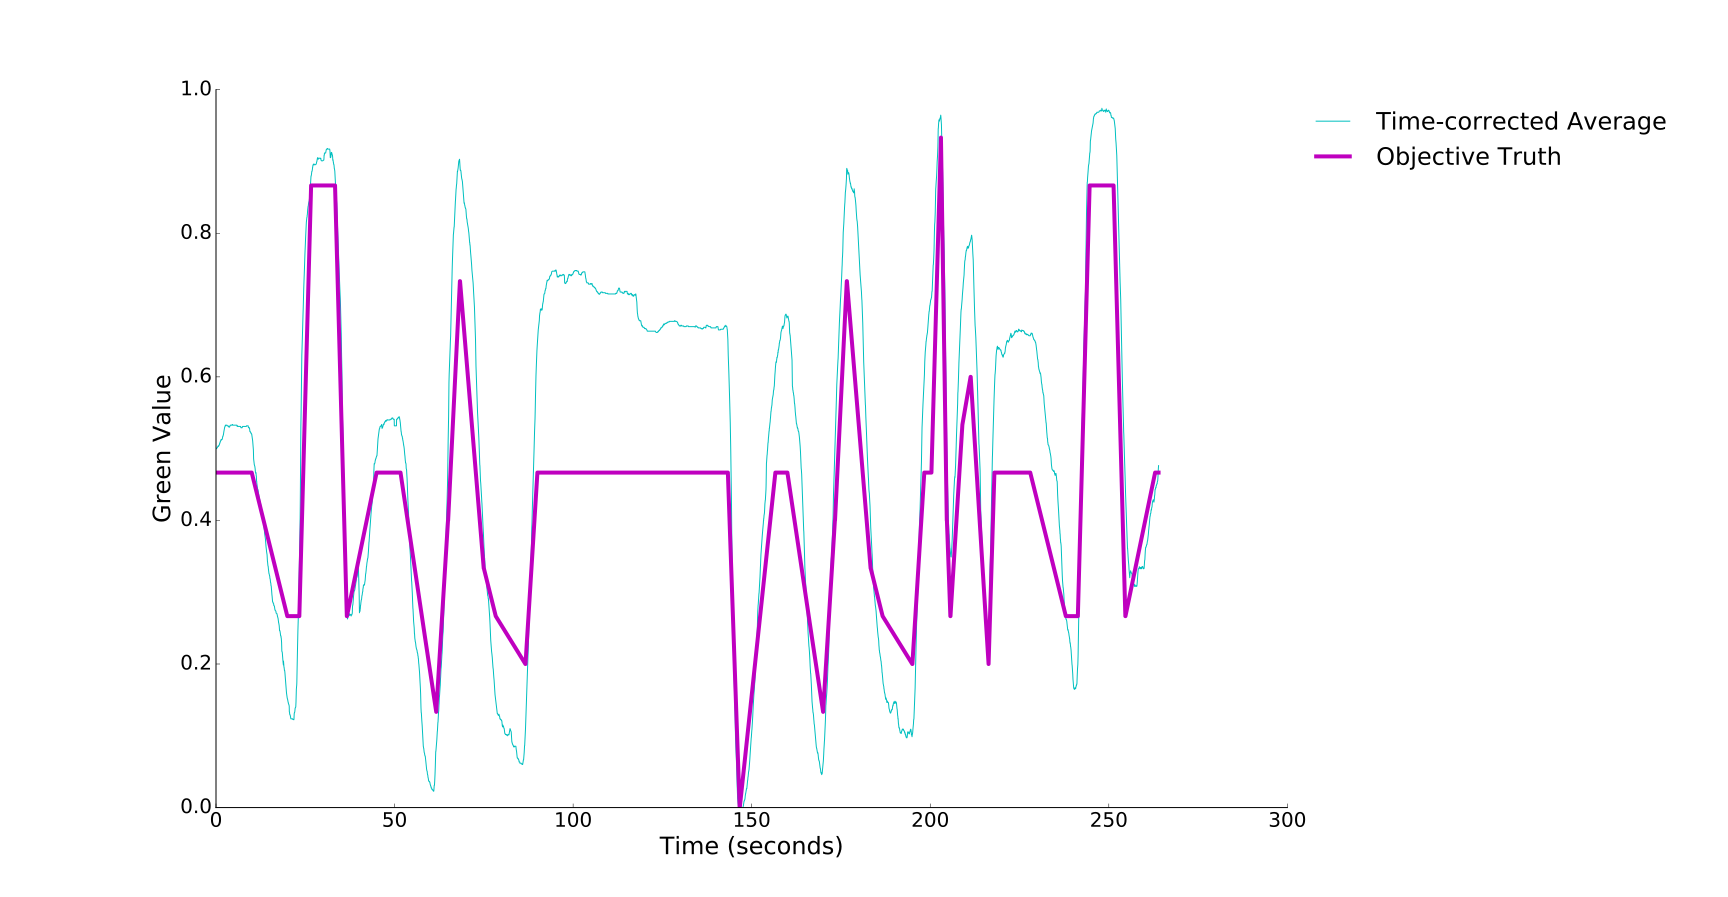
\includegraphics[width=\textwidth]{images/average_and_objective}
	\caption{Plot of time-corrected annotation average and objective truth.}
	\label{fig:average_and_objective}
	\end{subfigure}
	\begin{subfigure}{0.49\textwidth}
	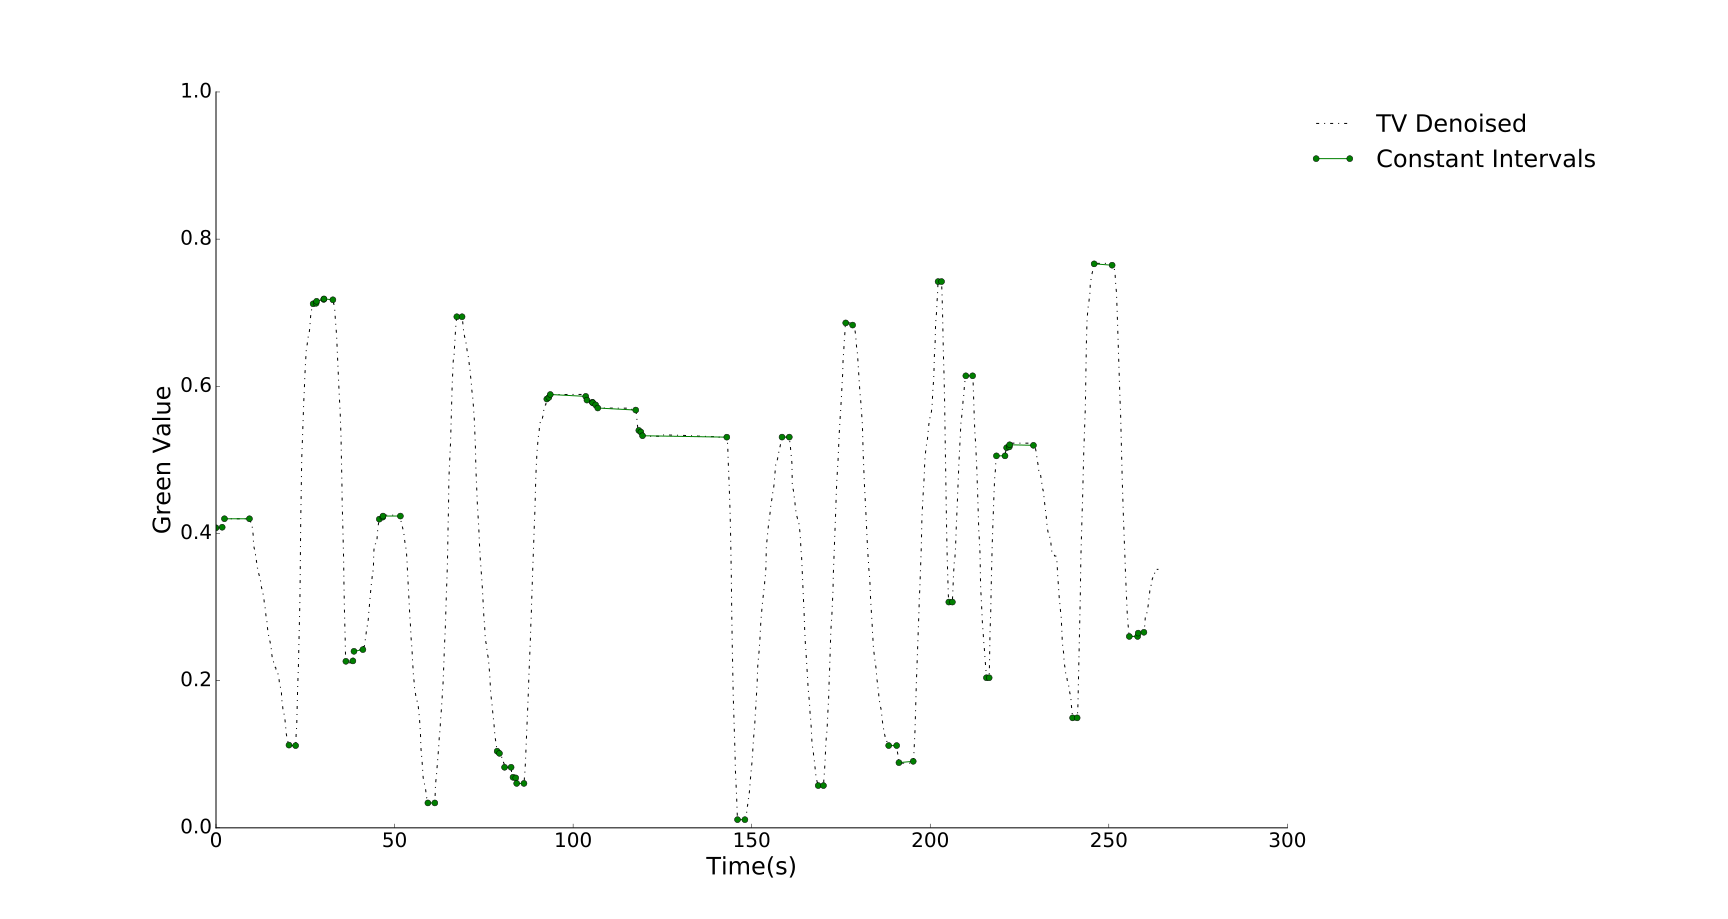
\includegraphics[width=\textwidth]{images/tv_and_intervals}
	\caption{Plot of TV-denoised fused annotation with extracted constant intervals.}
	\label{fig:tv_and_intervals}
	\end{subfigure}
	\caption{Results at intermediate stages of the proposed method pipeline for Task A.}
	\label{fig:average_and_objective_and_tv}
\end{figure*}

\subsection{Constant Interval Extraction}
A simple heuristic method is used to extract nearly constant intervals from the TV-denoised signal.  These time intervals become the targets for re-ranking in the next step when an ordinal embedding is applied.  In this step, a scan of the TV-denoised signal is performed and the smallest set of (largest) intervals is found where each interval satisfies two criteria: (1) the total height does not exceed threshold $h$, and (2) the frame length of the interval is at least $T$ frames.  Figure \ref{fig:tv_and_intervals} shows example extracted approximately constant intervals for one of the annotation tasks.

For our experiment, we select $h=0.005$ and $T=18$ frames (for 30Hz videos).  The height threshold is chosen to be very small relative to the size of the annotation scale so only very flat regions are considered.  Because TV denoising does well at approximating the signal as a piecewise-constant function, we find this step in the overall procedure is not very sensitive to $h$.  The $T$ value is selected to match the duration of the fastest change in the objective truth.  In practice, this parameter could be approximated from the average annotation signal or tuned manually, but should be set no smaller than the equivalent of 0.25 seconds, which is roughly the average human reaction time.  In the future, we hope to obviate these parameters to make this approach more scalable and robust.

\subsection{Triplet Comparisons}
In this step during an actual experiment, annotators are asked to view three extracted video segments corresponding to each unique triplet of intervals.  One video segment serves as a reference and the other two as test candidates and the annotator is instructed to select which of the two candidate video segments is most similar to the reference.  For the purpose of assessing the robustness of this approach to missing and conflicting comparison information, we simulate the comparison results using the objective truth as an oracle.  Further analysis of these effects are explored in the results section.

\subsection{Ordinal Embedding}
Ordinal embedding problems attempt to learn a (typically lower dimension) embedding that preserves a similarity relationship between subsets of data points.  Given a set of inputs $\mathcal{Z} = \{z_1,...,z_n\}$ with each $z \in \mathbb{R}^m$ and a set of similarity relations on 4-tuples from $\mathcal{Z}$ of the form $s(z_i,z_j) < s(z_k,z_l)$ where $\{i,j,k,l\}$ is a 4-subset of $\{1,2,...,n\}$, the goal is to find a set $\mathcal{X} = \{x_1,...,x_n\}$ with each $x \in \mathbb{R}^d$ such that:
\begin{equation*}
||x_i-x_j|| < ||x_k-x_l|| \Longleftrightarrow s(z_i,z_j) < s(z_k,z_l)
\end{equation*}
\noindent
for some norm on $\mathcal{X}$. For our application, we are interested in the case $i=k$ where we have ordinal comparisons in the form of triplets (i.e. sample $i$ is more similar to sample $j$ than $k$).  One reason to prefer this simplification of the general problem is that it reduces the cardinality of the set of all possible comparisons given $\mathcal{Z}$ and thus the amount of additional information we need.

A further reduction would be possible if we consider relationships of the form:
\begin{equation*}
||x_i|| < ||x_k|| \Longleftrightarrow ||z_i|| < ||z_k||
\end{equation*}
for unique index pairs $\{i,k\}$.  This setup supposes that it is possible to directly assign a value to each sample $z$ with respect to the target construct for the purpose of comparing two samples, but this may not always be possible.  In cases where multiple conflicting or ambiguous criteria exist, as in the annotation of smile strength \citep{Gupta2016}, such a scale may not exist or be too unintuitive for human annotators.  So, for generality of this procedure, we choose the triplet comparison approach.

With triplets, the total number of comparisons that can be made when $|\mathcal{Z}|=n$ is $n\cdot{n-1 \choose 2}$ which scales $\mathcal{O}(n^3)$.  Fortunately, there is considerable redundancy in the comparison information and only a small fraction is necessary to find an embedding close to the optimal embedding.  Prediction error bounds have already been derived for a noisy formulation of this triplet embedding problem \citep{jain2016finite}, nonetheless we expect that the number of comparisons must scale like $\mathcal{O}(dn\log(n))$ ($d=1$ in our experiment).

In our method, ordinal embedding is used to reorder the constant intervals to make them more self-consistent and rank-aligned with the objective truth.  Several triplet ordinal embedding solvers have been proposed \citep{agarwal2007generalized, tamuz2011adaptively, van2012stochastic, amid2015multiview}.  We employ the t-stochastic triplet embedding (t-STE) approach \citep{van2012stochastic} because, as the authors highlight, it aggregates similar points and repels dissimilar ones.  We also favor this approach because it prefers the simpler explanation that two points in the embedding are identical when no evidence suggests otherwise (Occam's Razor principle).  Figure \ref{fig:warp_evaldep} shows the embedding results for the extracted constant intervals that have been rescaled to the proper $[0,1]$ range and computed using a complete set of triplet comparisons from the oracle.  Note that the embedding only preserves the relative similarity relationships, so the embedding scale is expected to be off by a (unknown) monotonic transformation of the objective truth's scale.

\subsection{Spatial Warping}

In the final step, the fused annotation is spatially warped using the ordinal embedding results with the extracted constant intervals to rectify inconsistencies.  First, within the time frame of each interval the annotation is corrected so its average over the interval is equal to the corresponding embedding value.  Then, the annotation between two intervals is linearly scaled to align with the warped annotation at the neighboring intervals.  We select a linear inter-interval warping function because it avoids distorting the signal.  A formal definition is provided by Equations \ref{eqn:interval_difference} and \ref{eqn:warp} in Figure \ref{fig:equations}, and Figure \ref{fig:warp_evaldep} shows the results after applying this warping technique.

\begin{figure*}[!t]
\normalsize
%\setcounter{MYtempeqncnt}{\value{equation}}
\setcounter{equation}{0}
\begin{eqnarray}
\label{eqn:interval_difference}
S_t &=& 
\begin{cases}
\mathcal{E}_i - \frac{1}{|\mathcal{I}_i|}\sum\limits_{s \in \mathcal{I}_i} y_{s} & \exists \mathcal{I}_i \in \mathcal{I} : t \subseteq \mathcal{I}_i \\
0 & \text{else}
\end{cases} \\
\label{eqn:warp}
y_t' &=& 
\begin{cases}
y_t + S_t & \exists \mathcal{I}_i \in \mathcal{I} : t \subseteq \mathcal{I}_i \\
\Big(\frac{y_t-y_a}{y_b-y_a}\Big)(y_b + \mathcal{S}_{b^+}) + \Big(\frac{y_b-y_t}{y_b-y_a}\Big)(y_a + y'_{a^-}) & \exists [a,b] = \mathcal{J}_j \in \mathcal{J} : t \subseteq \mathcal{J}_j
\end{cases}
\end{eqnarray}
%\setcounter{equation}{\value{MYtempeqncnt}}
% IEEE uses as a separator
\hrulefill
% The spacer can be tweaked to stop underfull vboxes.
\vspace*{4pt}
\caption{Equations for our proposed spatial warping method. Let $\mathcal{I}$ and $\mathcal{E}$ be the ordered and corresponding sets of non-overlapping time intervals and embedding values respectively.  Define $S_t$ for each interval $\mathcal{I}_i \in \mathcal{I}$ and $i \in \{1,2,...,|\mathcal{I}|\}$ to be the difference between interval $i$'s average value and the corresponding embedding value.  Let $t \in \{1,2,...,T\}$ be a time index, $y_t$ denote the fused annotation signal, $y'_t$ denote the warped signal value, and $\mathcal{J}$ be the set of time ranges between the intervals in $\mathcal{I}$ ($\{1,2,...,T\} \setminus \cup_{i} \mathcal{I}_i$).  A subscript $+$ or $-$ denotes a time just before or after the associated time index.  Edge cases where the time indices fall outside of $\{1,...,T\}$ are handled using the average signal value at the boundary.}
\label{fig:equations}
\end{figure*}

\begin{figure*}
	\centering
	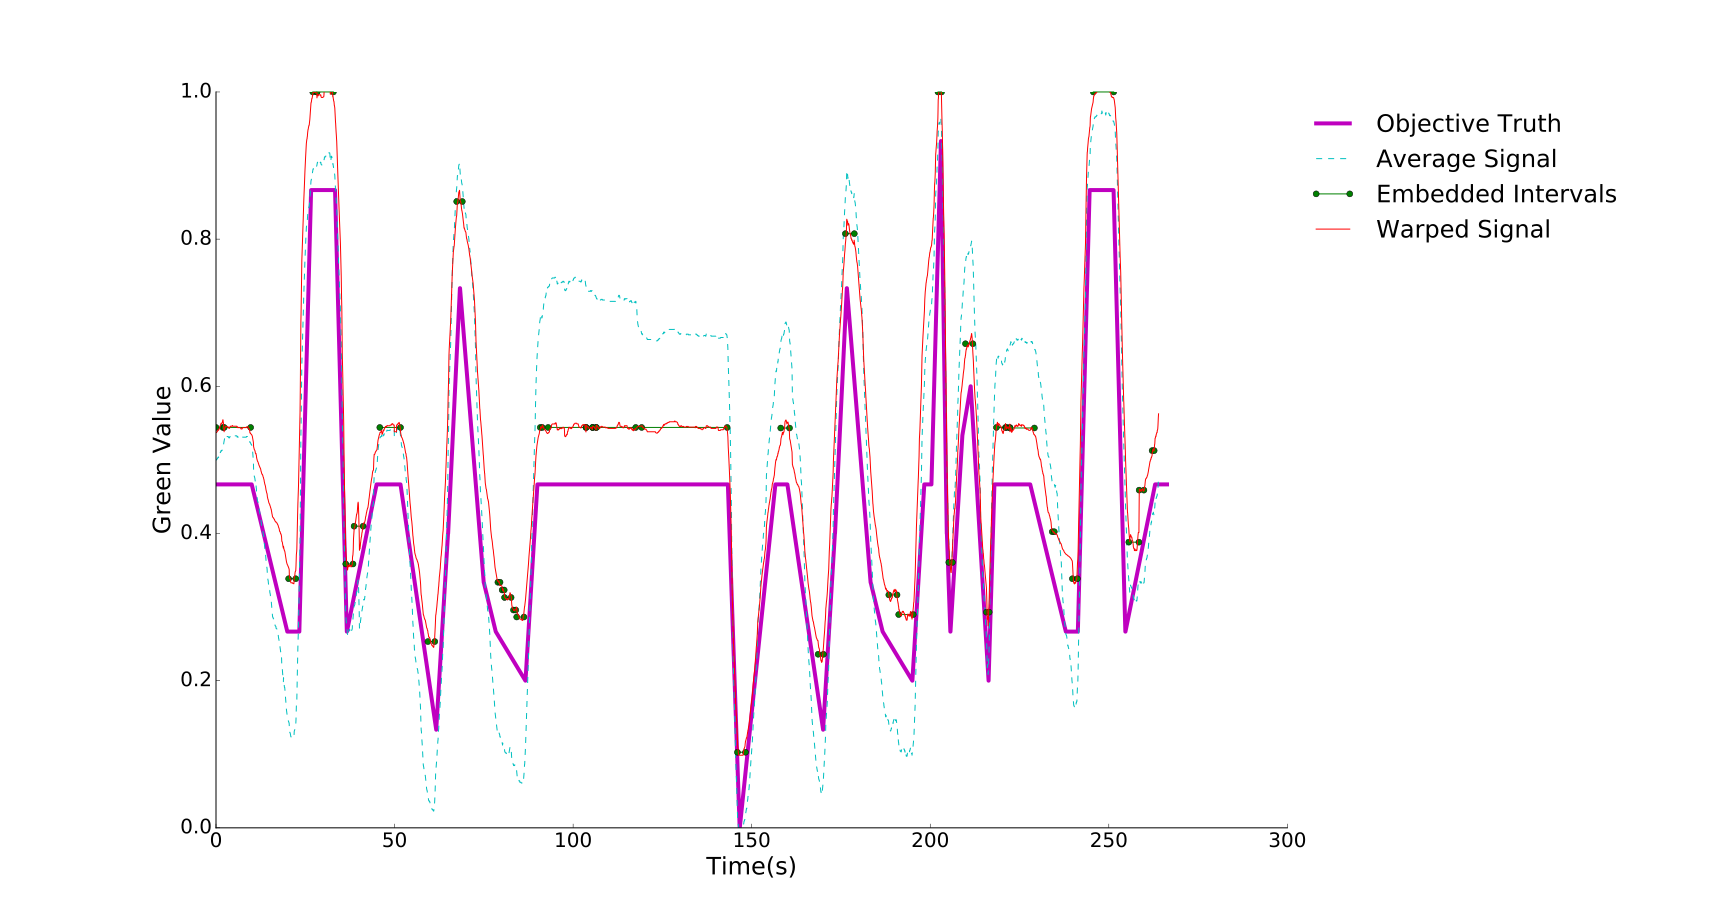
\includegraphics[width=0.8\textwidth]{images/warp_evaldep}
	\caption{Plot of the objective truth signal, time-shifted average annotation signal, warped signal, and the 1-D embedding for extracted constant intervals for Task A.  The spatially warped signal better approximates the objective truth and also achieves greater self-consistency over the entire annotation duration.}
	\label{fig:warp_evaldep}
\end{figure*}

\section{Results}
Table \ref{tab:results} shows various agreement measures for different annotation fusion approaches and the objective truth in our perception experiment.

\setlength\tabcolsep{1pt}
\setlength\extrarowheight{1pt}
\begin{table}[h!]
\caption{\label{tab:results} Agreement measures for baseline and proposed warped fused annotation approaches}
\centering
\begin{tabular}{ cccccc } 
 \Xhline{2\arrayrulewidth}
 \textbf{Task} & \textbf{Signal Type} & \textbf{Pearson} & \textbf{Spearman} & \textbf{Kendall's} & \textbf{NMI} \\
  & & & & \textbf{Tau} & \\
 \Xhline{2\arrayrulewidth}
 \multirow{6}{*}{\textbf{A}} & Simple Average & 0.775 & 0.795 & 0.636 & 0.302 \\ 
 & Warped Average & 0.811$^\dagger$ & 0.738 & 0.584 & 0.307 \\
 \cline{2-6}
 & Distort$^{*}$ & 0.809 & 0.834 & 0.676 & 0.793 \\
 & Warped Distort & 0.888$^\dagger$ & 0.839 & 0.695 & 0.794 \\
 \cline{2-6}
 & EvalDep$^{**}$ Average & 0.906 & 0.946 & 0.830 & 0.484 \\
 & Warped EvalDep & 0.967$^\dagger$ & 0.939 & 0.835 & 0.562 \\
 \Xhline{2\arrayrulewidth}
 \multirow{6}{*}{\textbf{B}} & Simple Average & 0.950 & 0.948 & 0.804 & 0.772 \\ 
 & Warped Average & 0.964$^\dagger$ & 0.960 & 0.828 & 0.859 \\
 \cline{2-6}
 & Distort$^{*}$  & 0.967 & 0.966 & 0.848 & 0.955 \\
 & Warped Distort  & 0.960 & 0.962 & 0.842 & 0.957 \\
 \cline{2-6}
 & EvalDep$^{**}$ Average  & 0.969 & 0.969 & 0.855 & 0.774 \\
 & Warped EvalDep  & 0.988$^\dagger$ & 0.987 & 0.906 & 0.862 \\
 \Xhline{2\arrayrulewidth}
\end{tabular}
\vspace*{4pt} \\
{\footnotesize All warped results use a complete set of ordinal comparisons from the oracle. NMI = normalized mutual information.  \\ $^\dagger$ - significant improvement ($p<0.005$, using a Fisher z-transform) of the warped methods over the respective signal \\ $^{*}$ - method from \cite{Gupta2016} \\ $^{**}$ - method from \cite{Mariooryad2015}}
\end{table}

Three baseline annotation fusions are shown, one is a simple average of the expert annotations, one is the maximum likelihood estimation from a per-annotator distortion model \citep{Gupta2016}, and the last is a time-aligned average using evaluator-dependent time shifts \citep{Mariooryad2015}.  Our rank-based warping method is applied to each baseline using a full set of triplet comparisons from the oracle.  In all cases except for one, the warping method achieves significantly better results ($p<0.005$) when agreement is measured using Pearson correlation or normalized mutual information.  In the one outlier case, the ``distort'' model already approximates the objective truth extremely well because the true signal is very smooth.  In this case, the proposed warping method does not diminish the correlation considerably.  Although it would seem that rank-based correlation metrics should show a substantial improvement, Spearman and Kendal's Tau correlations slightly decrease in some cases.  This is primarily due to rank disagreements over the warped constant intervals, rather than disagreements at a large scale due to the ordinal embedding.  The improved self-consistency over time of the warped signal combined with the general improvement in Pearson correlation demonstrate that the warped signal resulting from the proposed method is more suitable for use as a ground truth.

Lastly, we briefly address the robustness of the proposed warping method to incomplete triplet comparisons. Even for modest numbers of constant intervals, the number of triplets required for a complete set grows cubicly.  Due to the large amount of redundancy in the triplet comparisons, only a small fraction is necessary for the warping method to approximate the objective truth well.  Figure \ref{fig:warp_correlation_robustness} shows a plot of the performance of this spatial warping approach for both incomplete triplet comparisons and partially adversarial comparisons.  In our first green value perception experiment (Task A), there are 40 extracted intervals and thus 29,640 possible comparisons.  Assuming a uniform five percent triplet comparison error rate, significant improvement over the best tested baseline method is achieved with only two percent, or about 600, randomly selected triplet comparisons.

\begin{figure}
	\centering
	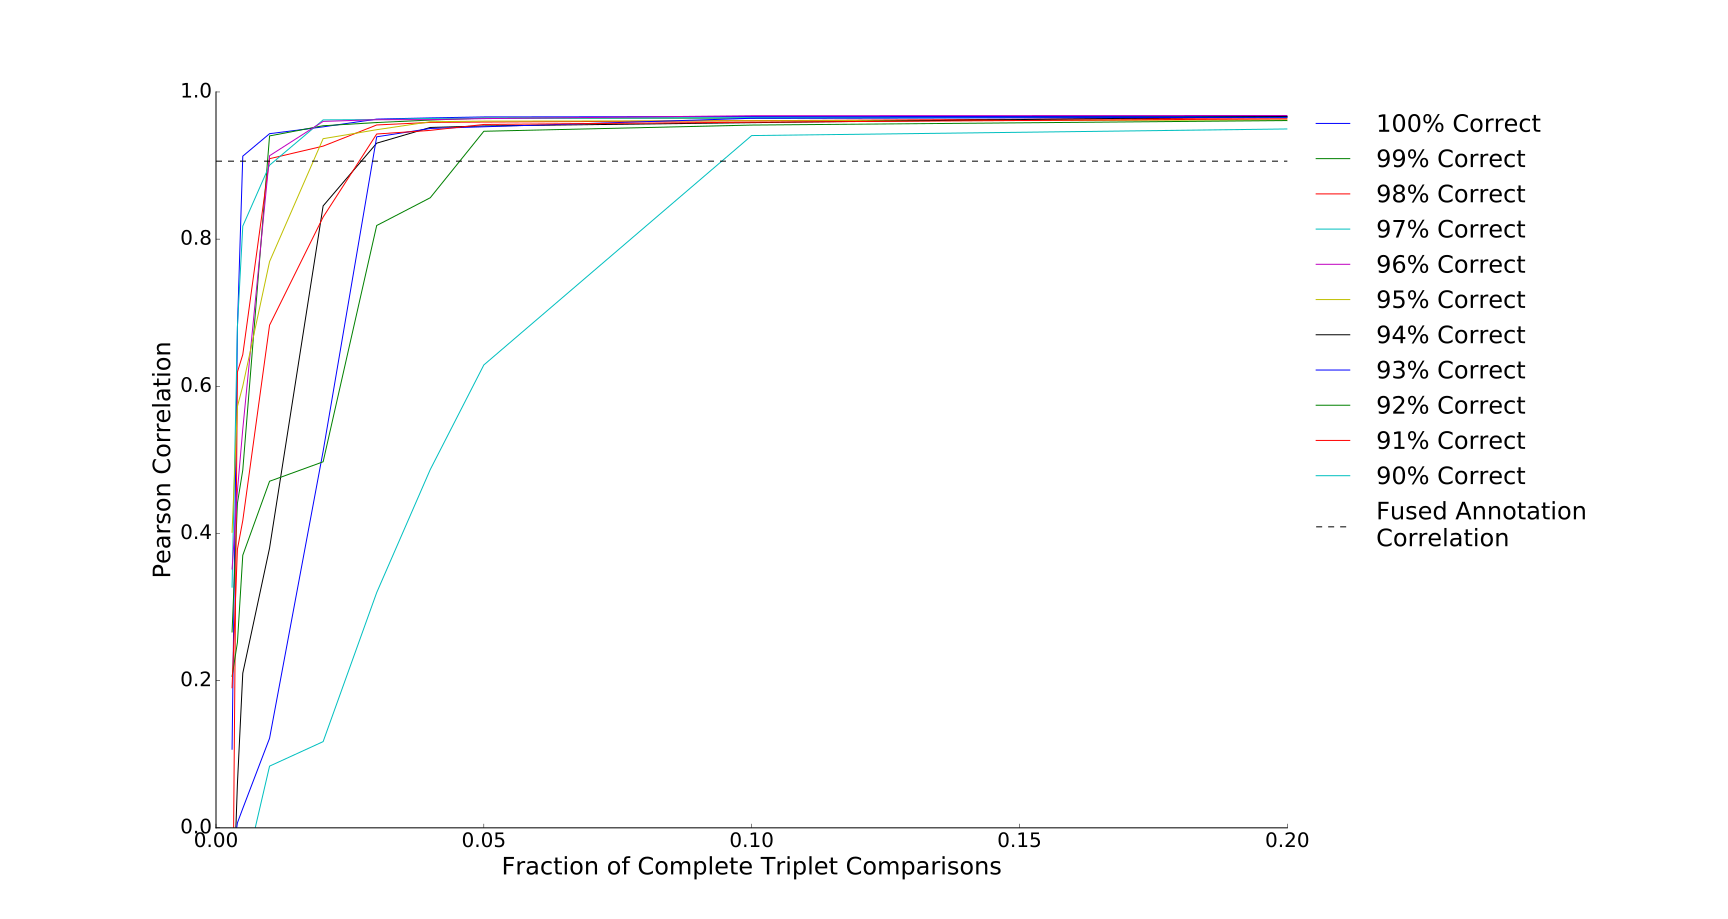
\includegraphics[width=\columnwidth]{images/warp_correlation_robustness}
	\caption{Plot showing Pearson correlation of the warped annotation (using Task A and the fusion from \cite{Mariooryad2015}) for different percentages of the total number of possible triplet comparisons.  Several plots are shown for varying levels of average annotation accuracy.  A high correlation is possible with a small fraction of the triplets due to large amounts of redundancy in the comparisons.}
	\label{fig:warp_correlation_robustness}
\end{figure}

\section{Future Work}
There are several compelling research directions for expanding on this work which we aim to address in future papers.  The total variation denoising procedure requires careful selection of an unintuitive tunable constant to achieve desirable results.  Consideration of other problem constraints, such as the quota of annotation resources available or the required accuracy on predictions from the resulting ground truth, could be used to find a sensible value for this parameter.  The subsequent constant interval extraction step also has two parameters that could be chosen automatically from the data given some additional heuristics or constraints.  Further analysis of this method's ability to produce accurate ground truth estimates for more complex continuous annotation tasks, like 2-D dimensional affect, is another exciting avenue.  Larger reductions in the number of required triplet comparisons may also be possible using adaptive sparse sampling techniques and stochastic transitivity.

\section{Conclusion}
In this paper we propose a novel method for extending continuous real-time human annotation fusion approaches to generate a more accurate ground truth.  We leverage the natural ability of annotators to provide accurate similarity comparisons and propose a procedure for warping the fused annotation to better align with the target construct.  We test our approach in a mechanically simple but perceptually difficult annotation experiment where an objective truth is known and show that our approach yields a signal significantly more correlated with the objective truth even with the presence of several annotation artifacts.  We hope this method finds utility as a means for establishing a more accurate ground truth in hidden state problems where no objective truth is available \textit{a priori}.

\bibliographystyle{model2-names}
\bibliography{sample}

\iffalse
\begin{table}[h!]
\centering
\begin{tabularx}{\textwidth}{ |K{1in}|C|C|C|C|C|C|C|C| } 
 \hline
 Annotation Artifact Sources & \multicolumn{8}{|c|}{Approximate Effect} \\
 \hline
 & Time shift & Mean bias & Variance bias & Local decoherence & Global decoherence & Decreased coherence & Improved coherence & Negative correlation \\
 \hline
 Human Reaction Lag & \X & & & & & & & \\ \hline
 System Input Processing Lag & \X & & & & & & & \\ \hline
 Input Errors & & & & \X & & & & \\ \hline
 Initial Input State & & \X & & & & & &\\ \hline
 Acclimation to Task & & & & & & & \X & \\ \hline
 Fatigue & & & & & & \X & & \\ \hline
 Iconic/Echoic memory duration & & & & & \X & & & \\ \hline
 Recalling similar annotation event & & & & \X & & & & \\ \hline
 Perception bias & & \X & \X & & & & & \\ \hline
 Experience bias & & \X & \X & & & & & \\ \hline
 Distractions & & & & \X & & & & \\ \hline
 Preoccupations / Mood & \X & \X & \X & \X & \X & & & \\ \hline
 Context bias & & \X & \X & \X & \X & & & \\ \hline
 Adversarial annotation & & \X & \X & \X & \X & & & \X \\ \hline
 Cognitive workload & \X & & & \X & & & & \\
 \hline
\end{tabularx}
\caption{Possible sources of annotation artifacts from a real-time continuous annotation process and the effect each has on the annotation signal.}
\label{tab:results}
\end{table}
\fi

\end{document}